\documentclass{beamer}

\usepackage[utf8]{inputenc}
\usepackage[spanish]{babel}

\usepackage{url}

% Más temas en
% http://deic.uab.es/~iblanes/beamer_gallery/index_by_theme.html
%\usetheme{Berlin}
%\usetheme{Copenhagen}
\usetheme{Warsaw}
%\usetheme{Darmstadt}

\setbeamercovered{transparent} %Items ocultos transparentes

\setbeamertemplate{background}{
  \rule{0pt}{.95\paperheight}%
  \hspace*{.98\paperwidth}%
  \makebox[0pt][r]{
\includegraphics[width=1.5cm]{fig/logo_fifa}}}

\title{Taller de Python}
\subtitle{Segundo encuentro: Numérico}
\author{FIFA}
\institute[FIFA]{Federación Interestudiantil de Física Argentina}
\date{24 de octubre de 2014}

%\AtBeginSubsection[]
%{
%  \begin{frame}<beamer>{Outline}
%    \tableofcontents[currentsection,currentsubsection]
%  \end{frame}
%}

% Let's get started
\begin{document}

\begin{frame}
  \titlepage
\end{frame}


\section{¿Por qué Python?}

\begin{frame}
    \frametitle{¿Por qué Python y no X?}
    Python es un \emph{lenguaje de programación}:
    \begin{itemize}
    \item Libre
    \item Expresivo
    \item Mucho soporte de la comunidad
    \item Divertido. 
    \end{itemize}
    Además, a diferencia de otros lenguajes es \emph{interactivo} (si uno sabe usarlo)
\end{frame}


\section{¿Con qué programo Python?}

\subsection{Compilador, IDE, y todo eso}

\begin{frame}[fragile]{¿Qué necesito para programar Python?}
  \begin{onlyenv}<+>
 Como todo lenguaje, la computadora y vos necesitan un diccionario, lo que se llama \emph{compilador}. Sobre ese compilador, en general se distribuye parte de programas hecho por otras personas, que en conjuto se llaman \emph{librerías}.
 \end{onlyenv}
 \begin{onlyenv}<+>
 Para eso, podemos instalar Anaconda, que instala todos los programas que vamos a usar (compilador) y librerías. Además, instala algunos programas para ayudarnos a escribir Python, denominados IDE. Nosotros vamos a usar el programa \emph{Spyder}.
 \end{onlyenv}
 \begin{onlyenv}<+>
    Páginas de los programas necesarios
    \begin{itemize}
    \item{Anaconda \url{http://continuum.io/downloads#py34}}
    \item{Miniconda (Anaconda sin librerías, ni programas) \url{http://conda.pydata.org/miniconda.html}}
    \item{Spyder \url{http://goo.gl/VByA2t}}
    \end{itemize}
 \end{onlyenv}
 \begin{onlyenv}<+>
    Comandos útiles de teclado de Spyder
    \begin{itemize}
    \item F5: Ejecutar archivo editado
    \item Shift + Ctrl + E: Ir a editor
    \item Shift + Ctrl + C: Ir a consola
    \item Tab: autocompletar (en consola también!!)
    \end{itemize}
 \end{onlyenv}
\end{frame}

\section{Cálculo numérico}

\subsection{¿Para qué cálculo numérico?}
\begin{frame}
    \frametitle{Cálculo numérico... ¿y eso?}
    En esta época donde las computadoras son ubicuas, la ciencia avanza sobre el cálculo numérico:
    \begin{itemize}
    \item Realizar y analizar mediciones antes imposibles (imaginen el LHC sin computadoras!!);
    \item Prototipando la realidad con simulaciones.
    \end{itemize}
    Obviamente que esta el argumento básico, resolver problemas puros numéricos, pero queremos tener una aplicación para aprender a usarla.
    
\end{frame}

\subsection{Objetivos de cálculo numérico}

\begin{frame}{Objetivos del cálculo numérico}

    El objetivo del cálculo numérico:
    \begin{itemize}
    \item Determinar diferentes algoritmos para el mismo problema;
    \item Determina la cantidad de pasos a realizar, por lo tanto la velocidad al ejecutarse;
    \item Determinar el error que se comete al efectuar una cantidad determinada de iteraciones.
    
    \end{itemize} 

\end{frame}

\subsection{Problemas del cálculo numérico}

\begin{frame}[fragile]{Problemas del cálculo numérico}


\uncover<+>{Como la computadora \emph{no} tiene infinita memoria, \emph{no existe} forma de representar los números reales.}

\uncover<+>{
Para eso existen los números de punto flotante (llamados float), tienen precisión y cota. Prueben sumar 0,1 y 0,2}

\uncover<+>{El ejemplo anterior es claro: hay que tener cuidado con la aritmética de floats, puede dar errores groseros al sumar a un número grande uno muy pequeño, o al dividir por algún número muy pequeño, o el error intrínseco de la representación.}

\end{frame}

\begin{frame}[fragile]{Problemas del cálculo numérico II}

Y en general para comparar floats se debe tomar una cota de error plausible, es decir
\begin{verbatim}
 In [2]: a = 0.1; b = 0.10000001
 In [3]: if a - b < 0.00001:
 .... print(True)
 True
\end{verbatim}

\end{frame}

\section{Numpy, arrays y esas yerbas}

\subsection{Numpy, ¿qué es eso?}

\begin{frame}[fragile]{Numpy, ¿qué es eso?}
    Numpy es la librería básica para el análisis numérico. Antes de ver de qué se trata, hagamos una prueba de fuego.

Para eso probemos ingresando lo siguiente en la consola
    \begin{verbatim}
     In [1]: import numpy as np
     In [2]: A = np.array([[1,2],[3,4]])
     In [3]: A
     Out [1]: array([1,2]
                    [3,4])
    In [4]: A[1,1]
    Out [2]: 4
    \end{verbatim}
\end{frame}

\begin{frame}{Ventajas de Numpy}
    \begin{itemize}
    \item Implementado sobre lenguajes de bajo nivel (C/C++, Fortran)
    \item Es \emph{muy} rápido (más que Matlab)
    \item Tiene casi toda la funcionalidad que se usa en los ambientes científicos y tecnológicos.
    \end{itemize}
\end{frame}

\subsection{Programas simples con Numpy}


\begin{frame}[fragile]{Python: Calculadora avanzada}
    Hagamos algunas cuentas con Numpy
    \begin{verbatim}
    In [1]: 5 * 5
    Out [1]: 15
    In [2]: np.sin(np.pi/2)
    Out [2]: 1
    In [3]: np.exp(2)
    Out [3]: 7.3890560989306504
    \end{verbatim}
\end{frame}

\begin{frame}[fragile]{Cálculo con matrices}
    
    \begin{onlyenv}<+>
    Prueben lo siguiente
    \begin{verbatim}
    In [5]: B = np.array([[3,1,2],[1,4,1],[2,1,5]])
    In [6]: import numpy.linalg as lin
    In [7]: lin.eig(B)
    Out[3]: 
    (array([ 6.89510652,  1.70759841,  3.39729507]),
     array([[ 0.49725362,  0.86427949,  0.07589338],
            [ 0.43170413, -0.17059871, -0.88573564],
            [ 0.75257583, -0.47319874,  0.45794385]]))
    \end{verbatim}
    Eig de eigenvalues/eigenvectors, autovalores. Todos sabemos que son cosas útiles.
    \end{onlyenv}
    \begin{onlyenv}<+>
    Solucionemos un sistema lineal $Bx=b$.
    
    Acordate que todavía tenés definida B, así que definamos b:
    
    \begin{verbatim}
        In [8]: b = np.array([2,0,1])
        In [9]: lin.solve(B,b)
        Out[4]: array([ 0.775, -0.175, -0.075])
    \end{verbatim}
    
    \end{onlyenv}
    
\end{frame}


\section{Yendo un poco más serio}
\begin{frame}[fragile]{}
 Para las diapositivas que vamos a ver a continuación tenemos que ejecutar previamente el siguiente comando
 \begin{verbatim}
 import numpy as np
 import scipy as sp
 import scipy.optimize as opt
 import matplotlib.pyplot as plt
 \end{verbatim}
 que representan los paquetes que vamos a utilizar. 
 
 Y como ya estamos más grandes, trabajemos directamente en el editor, y con F5 ejecutemos el código escrito en consola. 
 
 \emph{Así se trabaja generalmente}
\end{frame}

\subsection{Obtención de raices}

\begin{frame}[fragile]{Obtención de raíces}
    Ahora vamos a encontrar la raíz de una $f(x)$.
    Primero debemos definirla. Usemos la definición \emph{inline}
    
    \begin{verbatim}
    f = lambda x: np.log(x) - 1
    x0 = 3
    print(opt.newton(f, x0))
    #2.71828182846
    \end{verbatim}
    
\end{frame}

\subsection{Ajustes de datos}

%%%%%%% revisar esta diapo

\begin{frame}[fragile]{Ajustes de datos}
    Primero creamos los datos. \emph{En general} se obtienen de una experiencia, pero como ejemplo usamos un algoritmo aleatorio para obtenerlos.
    
    \begin{onlyenv}<+>
    Para eso definamos una función que determina el modelo
    
    \begin{verbatim}
    def f(p,x):  
    return p[0]*x/np.sqrt(p[1]*x**2 + 
           (x**2 - p[2]**2)**2)
    \end{verbatim}
    
    \end{onlyenv}
    
    \begin{onlyenv}<+>
    
    \begin{verbatim}
x = np.linspace(0,5,70)
y = f([2,4,2],x) + np.random.random(x.size)*0.05 - 0.025
np.savetxt("datos.csv",np.array([x,y]).T)
\end{verbatim}
    
   De esta forma en el archivo datos.csv está la tabla de datos
   \end{onlyenv}
\end{frame}

\begin{frame}[fragile]{Ajustes de datos}
    Ahora creamos una variable data con los datos guardados en datos.csv. También creamos los errores dx y dy con un algoritmo.
    \begin{verbatim}
    data = np.loadtxt("datos.csv")
    dx = np.ones_like(data[:,0])*0.02
    dy = np.ones_like(data[:,1])*0.05
   \end{verbatim}
   
\end{frame}

\begin{frame}[fragile]{Ajustes de datos}
    Finalmente ajustamos con la librería scipy.odrpack, que tiene una función especializada en Regresión ortogonal (con errores en ambas variables)
    \begin{verbatim}


beta0 = [1,1,1] #Parametros iniciales
out = sp.odr.odrpack.odr(f, beta0, y, x, 
                         full_output = 1)
print(out[0],out[1],out[3]['sum_square'])
\end{verbatim}
   
\end{frame}


\subsection{Visualización de datos}

\begin{frame}[fragile]{Visualización de datos}
\begin{onlyenv}<+>
    Ahora que tenemos todos los datos analizados, queremos visualizarlos. Para eso usamos la librería matplotlib, con su módulo pyplot. Este módulo nos permite usar funciones simples para imprimir gráficos
\begin{verbatim}
import matplotlib.pyplot as plt
plt.errorbar(x,y,dy,dx,'.r')
plt.plot(x,f(out[0],x))
plt.show()
\end{verbatim}
\end{onlyenv}
\begin{onlyenv}<+>
  \begin{figure}
  \centering
  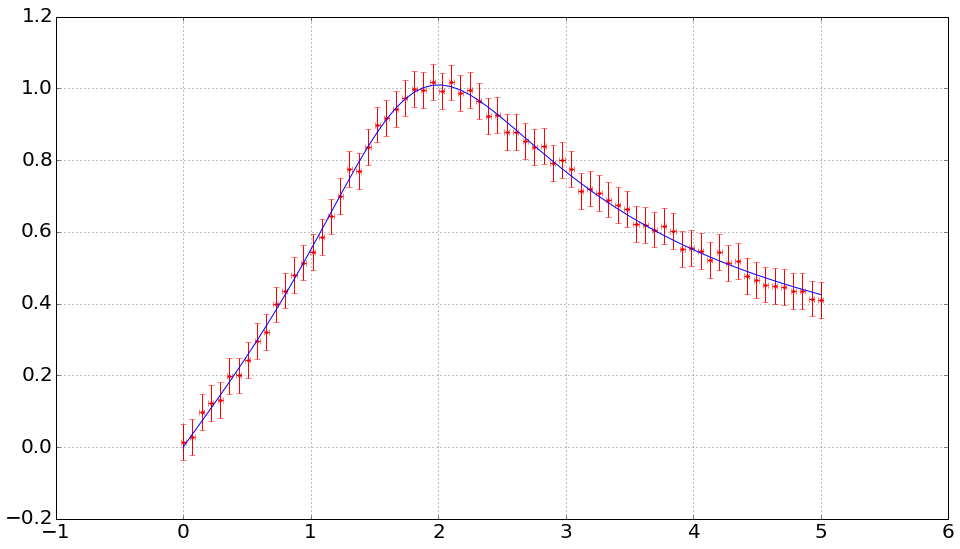
\includegraphics[width=0.8\textwidth]{fig/fit}
  \label{fig:fit}
  \end{figure}
\end{onlyenv}
\end{frame}

\subsection{Integración de ODE}

\begin{frame}[fragile]{Integración de ODE}
\begin{onlyenv}<+>
Para resolver una ecuación diferencial ordinaria (ODE), primero nos conviene definir la función $f(t,x) = x'$, la expresión funcional de la ODE
\begin{verbatim}
def van_der_pol(x,t,mu):
#Oscilador de Van Der Pol
    X, Xdot = x 
    return [Xdot, mu*(1-X**2)*Xdot - X]
\end{verbatim}
\end{onlyenv}
\begin{onlyenv}<+>
    Con eso podemos pasar a definir la escala de tiempo, los parámetros del problema y las condiciones iniciales

\begin{verbatim}
x0 = [0,1] #Condiciones iniciales
t = arange(0,50,0.01)
mu = 5 #Parámetro
p = (mu,)  #Si le pasa (mu) no agarra como tupla
\end{verbatim}

\end{onlyenv}
\begin{onlyenv}<+>
   Para que finalmente ejecutemos el integrador, que para Python usa Runge Kutta de orden 4 u 5 dependiendo de los parámetros finos del método
   \begin{verbatim}
sol = sp.integrate.odeint(van_der_pol,x0,t,args=p)
   \end{verbatim}
\end{onlyenv}

\begin{onlyenv}<+>
Si queremos representar el resultado, usamos nuevamente la librería matplotlib.pyplot, pero con el siguiente código
\begin{verbatim}
plt.figure(1,figsize=(16,9))
plt.subplot(1,2,1)
plt.plot(t,sol[:,0]) #Posición
plt.subplot(1,2,2)
plt.plot(sol[:,0],sol[:,1]) #Diagrama de fase
plt.show()
\end{verbatim}
\end{onlyenv}

\begin{onlyenv}<+>
Y acá está el resultado
\begin{figure}
  \centering
  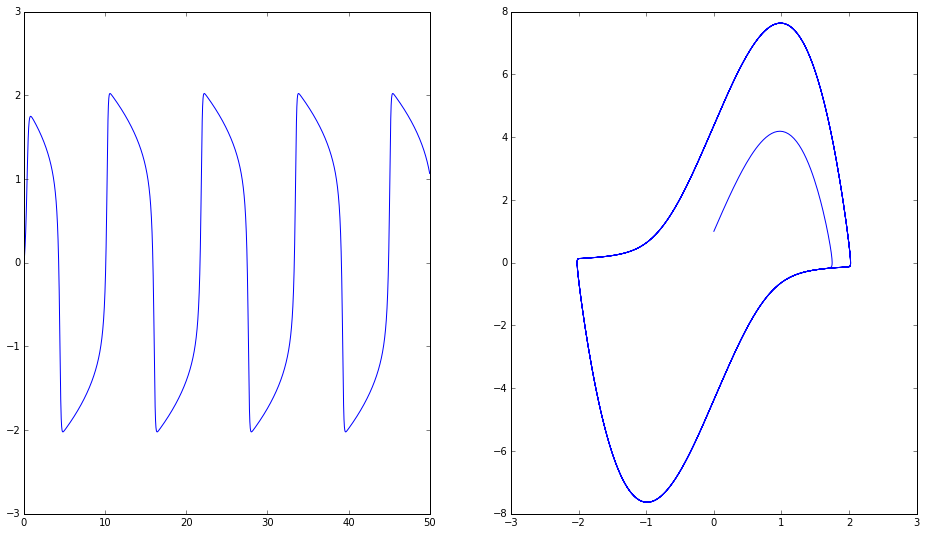
\includegraphics[width=0.8\textwidth]{fig/ode}
  \label{fig:ode}
  \end{figure}
\end{onlyenv}

\end{frame}



\end{document}
